\documentclass{beamer}
%-----------------------------------------------------------------------------%
\usepackage{settings-color}
\usepackage{settings}
\usepackage{settings-math}
\usepackage{settings-algorithm}
\usepackage{settings-cjk}
\usepackage{settings-gloss}
\usepackage{settings-biblatex}
\usepackage{settings-tables}
%-----------------------------------------------------------------------------%
%%% Title %%%
\title{A Bayesian Approach to\\the Problem of Unknown Networks\\in Spatial Autoregressive Models}
\author{陳\,捷\\Jesse Chieh Chen}
\date{\texttt{2024-05-24}}
%-----------------------------------------------------------------------------%

\begin{document}

\maketitle

\begin{frame}{Contents}
	\tableofcontents
\end{frame}

\section{Introduction}

\begin{frame}{Motivation}
	\begin{itemize}
		\item
			Econometricians are interested in networks,
			but network data are hard to come by.
		\item
			In many cases,
			although the network structure is unknown,
			we have a good idea about its characteristics (e.g., small world, mutuality).
	\end{itemize}
	\begin{block}{Question}
		How can we effectively incorporate these characteristics in estimation?
	\end{block}
\end{frame}

\begin{frame}{Literature}
	In other fields:
	\begin{itemize}
		\item Causal Inference:
			\begin{enumerate}
				\item \cite{madigan-1994}: \acrshort{dag} causal graph recovery
				\item \cite{yuan-2007}: recover covariance relations
			\end{enumerate}
	\end{itemize}
	In Econometrics:
	\begin{itemize}
		\item Frequentist attempts: High-dimensional Methods
			\begin{enumerate}
				\item \cite{meinshausen-2006}: Lasso
				\item \cite{lam-2020}: Lasso
				\item \cite{de_paula-2023}: Identification without sparsity, elastic net
			\end{enumerate}
		\item Bayesian attempt: \cite{krisztin-piribauer-2022}
			\begin{enumerate}
				\item
					Simple network priors (\acrlong{er} type)
				\item
					No motivation from network formation
			\end{enumerate}
	\end{itemize}
\end{frame}

\section{Model Setup}

\begin{frame}{\acrlong{sar}}
	\begin{block}{\acrshort{sar}}
		\vspace{-1em}
		\begin{align*}
			\underset{(N\times 1)}{\yy}
			= \lambda\underset{(N\times N)}{\bar\WW}\yy
			+ \underset{(N\times K_1)}{\XX_{1}}\underset{(K_1\times 1)}{\bbeta_1}
			+ \bar\WW\XX_{2}\underset{(K_2\times 1)}{\bbeta_2}
			+ \uu
		\end{align*}
	\end{block}
	\begin{itemize}
		\item $\yy$: vector of outcome variables
		\item $\bar\WW$: row-normalized adjacency matrix
		\item $\XX_{1},\XX_{2}$: exogenous variables
		\item $\uu$: Gaussian error
	\end{itemize}
	\begin{enumerate}
		\item $\lambda$: peer effect or endogenous effect
		\item $\bbeta_1$: exogenous effect
		\item $\bbeta_2$: contextual effect
	\end{enumerate}
\end{frame}

\begin{frame}{Why Bayesian?}
	\begin{itemize}
		\item
			There are two problems with \acrshort{sar}:
			\begin{enumerate}
				\item The network is endogenously formed
				\item The network is, in many cases, unknown
			\end{enumerate}
		\item
			It is natural to specify a \textbf{network formation model}.
		\item
			Hence, the likelihood combined with the network formation probability gives the \textbf{complete} picture.
		\item
			This calls for a Bayesian approach.
			\begin{align*}
				% \pr(\WW\given\lambda,\bbeta_1,\bbeta_2)
				% \propto
				\underset{\text{\acrshort{sar} likelihood}}{f(\yy\given\lambda,\WW,\bbeta_1,\bbeta_2)}
				\cdot
				\underset{\substack{\text{network}\\\text{formation}}}{\pr(\WW)}
			\end{align*}
		\item
			In this research, we focus on \acrshort{ergm} priors.
	\end{itemize}
\end{frame}

\begin{frame}{\acrlong{ergm}}
	\begin{block}{\acrshort{ergm}}
		\vspace{-1em}
		\begin{align*}
			\pr(\WW\given\ttheta) = \frac1{z(\ttheta)} \exp(\ss(\WW)\T\ttheta)
			\hspace{0.5em}\text{where}\hspace{0.5em}
			z(\ttheta) = \sum_{\tilde\WW\in\WWW} \exp(\ss(\tilde\WW)\T\ttheta)
		\end{align*}
	\end{block}
	\begin{itemize}
		\item $\ss(\WW)$: vector of sufficient statistics,
		\item $\ttheta$: vector of natural parameters
		\item $z(\ttheta)$: normalizing constant.
	\end{itemize}
	\vspace{1em}
	\begin{enumerate}
		\item \blue{Flexibility:} $\ss(\ttheta)$ can be anything
			\begin{itemize}
				\item \acrlong{er} (Poisson), homophily models, etc
			\end{itemize}
		\item \blue{Tractability:} known algorithms to sample $\WW$ and recover $\ttheta$
		\item \blue{Interpretability:} some microfoundation
	\end{enumerate}
\end{frame}

\section{Model Specifications}

\begin{frame}{Likelihood Function}
	\begin{align*}
		&\raum f(\yy\given\lambda,\WW,\bbeta,\sigma^2) \\
		&=
		(2\pi)^{-N/2}
		(\sigma^2)^{-N/2}
		\det(\MM)
		\exp \left( -\frac1{2\sigma^2} \norm{\MM\yy - \HH\bbeta} \right)
	\end{align*}
	\begin{itemize}
		\item $\bbeta$ is the vector of parameters $(\bbeta_1,\bbeta_2)\T$
		\item $\MM$ is the reduced form matrix $\II-\lambda\WW$
		\item $\HH$ is the stacked exogenous variables $[\XX_{1},\WW\XX_{2}]$
		\item $\norm{\xx}$ is the Euclidean norm $\xx\T\xx$
	\end{itemize}
\end{frame}

\begin{frame}{Priors}
	\begin{center}
		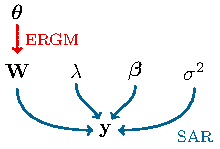
\includegraphics[width=0.35\textwidth]{figures-tikz/ergm.pdf}
	\end{center}
	\begin{block}{}
		\vspace{-1em}
		\begin{align*}
			\begin{cases}
				\bbeta                & \sim \Normal(\mmu_{\bbeta},\VV_{\bbeta}) \\
				\sigma^2              & \sim \InverseGamma(a_{\sigma^2},b_{\sigma^2}) \\
				\lambda               & \sim \Uniform(-1,1) \\
				\pr(\WW\given\ttheta) & \propto \exp(\ss(\WW)\T\ttheta) \hspace{5em}\text{(\acrshort{ergm})} \\
				\ttheta               & \sim \Normal(\mmu_{\ttheta},\VV_{\ttheta})
			\end{cases}
		\end{align*}
	\end{block}
\end{frame}

\begin{frame}{Priors: Panel Data}
	\begin{center}
		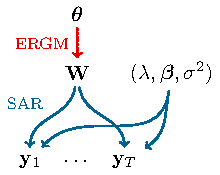
\includegraphics[width=0.35\textwidth]{figures-tikz/ergm-panel.pdf}
	\end{center}
	\begin{itemize}
		\item
			One observation of $\yy$ contains too little information.
		\item
			We assume we have iid observations $\{\yy_{t},\XX_{t}\}$ with likelihood function:
			\begin{align*}
				f(\{\yy_{t}\}\given\lambda,\WW,\bbeta,\sigma^2)
				= \prod_{t} f_t(\yy_{t}\given\lambda,\WW,\bbeta,\sigma^2)
			\end{align*}
	\end{itemize}
\end{frame}

\section{Sampling Procedure}

\begin{frame}{Sampling: $\bbeta$ and $\sigma^2$}
	\begin{itemize}
		\item
			With prior $\bbeta\sim\Normal(\mmu_{\bbeta},\VV_{\bbeta})$,
			the posterior of $\bbeta$ also follows normal distribution.
			(Normal-Normal conjugacy)
		\item
			With prior $\sigma^{2}\sim\InverseGamma(a_{\sigma^2},b_{\sigma^2})$,
			the posterior density of $\sigma^2$ also follows Inverse Gamma distribution.
			(Inverse Gamma-Normal conjugacy)
	\end{itemize}
\end{frame}

\begin{frame}{Sampling: $\lambda$}
	The posterior density of $\lambda$ assumes no well-known form.
	With prior $\lambda\sim\Uniform(-1,1)$,
	the posterior density of $\lambda$ is proportional to the likelihood function:
	\begin{align*}
		\pr(\lambda\given\{\yy_{t}\},\WW,\bbeta,\sigma^2,\ttheta)
		&\propto f(\{\yy_{t}\}\given\lambda,\WW,\bbeta,\sigma^{2}) \\
		&= \prod_{t} f(\yy_{t}\given\lambda,\WW,\bbeta,\sigma^{2}).
	\end{align*}
	\begin{itemize}
		\item
			A simple \acrlong{mh} is used to sample posterior $\lambda$.
		\item
			One can also use \acrlong{gg}.
	\end{itemize}
\end{frame}

\begin{frame}{Sampling: $\WW$}
	The posterior probability of $\WW$ assumes no well-known form,
	it is proportional to
	\begin{align*}
		&\mathrel{\phantom{\propto}} \pr(\WW\given\{\yy_{t}\},\lambda,\bbeta,\sigma^{2},\ttheta) \\
		&\propto f(\{\yy_{t}\}\given\lambda,\WW,\bbeta,\sigma^{2}) \pr(\WW\given\ttheta) \\
		&\propto
		\det(\MM)
		\exp\left( -\frac1{2\sigma^2} \sum_{t} \norm{\MM\yy_{t}-\HH_{t}\bbeta} \right)
		\exp(\ss(\WW)\T\ttheta).
	\end{align*}
	\begin{itemize}
		\item
			Since this is a high-dimensional sampling problem,
			we use a discrete variant of \acrlong{hmc} to sample posterior $\WW$.
	\end{itemize}
\end{frame}

\begin{frame}{Sampling: $\ttheta$}
	The posterior density of $\ttheta$ assumes no well-known form,
	it is proportional to
	\begin{align*}
		&\mathrel{\phantom{\propto}} \pr(\ttheta\given\{\yy_{t}\},\lambda,\WW,\bbeta,\sigma^2) \\
		&\propto \pr(\WW\given\ttheta)\pr(\ttheta) \\
		&\propto
		\frac1{z(\ttheta)}
		\exp(\ss(\WW)\T\ttheta)
		\exp\left(-\frac12(\ttheta-\mmu_{\ttheta})\T\VV_{\ttheta}\inv(\ttheta-\mmu_{\ttheta})\right).
	\end{align*}
	\begin{itemize}
		\item
			Since $z(\ttheta)$ is unknown,
			we use \acrlong{ex} to obtain posterior samples of $\ttheta$.
	\end{itemize}
\end{frame}

\begin{frame}[fragile]{Gibbs Sampling}
	\begin{block}{}
		../paper/algorithmic-gibbs.tex
	\end{block}
	\begin{itemize}
		\item
			All sampling algorithms are implemented in \texttt{R} and \texttt{C++}
	\end{itemize}
\end{frame}

\section{Simulation}

\subsection{Basic \acrshort{ergm}}

\begin{frame}{Basic \acrshort{ergm}}
	\begin{center}
		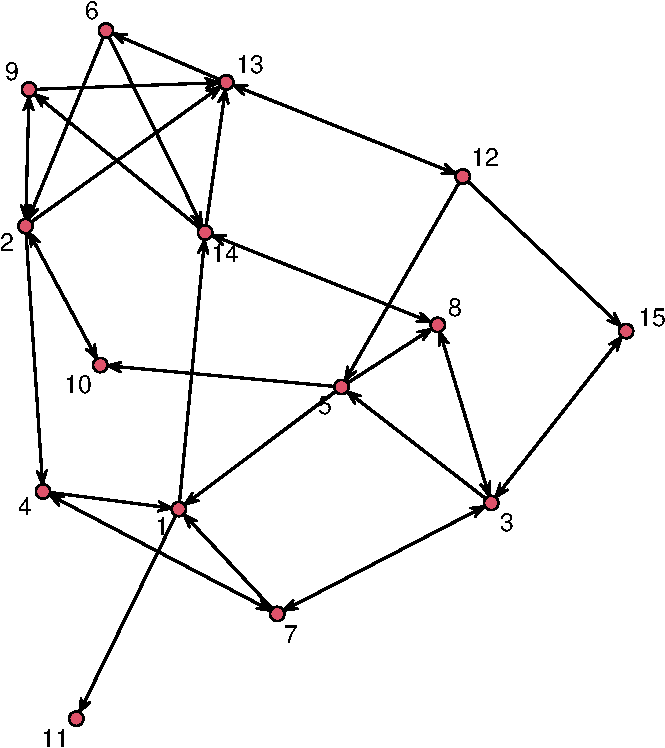
\includegraphics[width=0.40\textwidth]{figures/penta.pdf}
		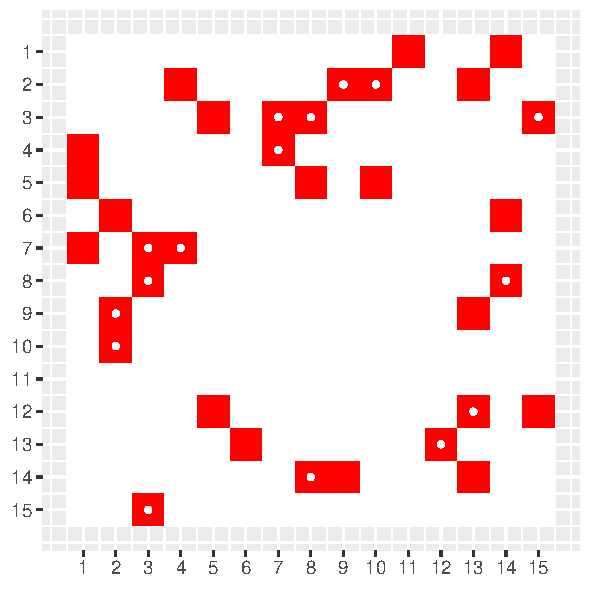
\includegraphics[width=0.45\textwidth]{figures/penta-W.pdf}
	\end{center}
	\begin{itemize}
		\item
			This network is generated from \acrshort{ergm} with
			$\text{\texttt{edges}}=-2$ and
			$\text{\texttt{mutual}}=2$.
		\item
			Simulated data is generated for $T=12$.
	\end{itemize}
\end{frame}

\begin{frame}{Group P1 and P2}
	\begin{itemize}
		\item\blue{\textbf{Group P1}}:
			$\XX_1$ is an $N\times 1$ matrix of exogenous variables generated from a normal distribution and $\XX_{2}$ equals $\XX_{1}$.
		\item\blue{\textbf{Group P2}}:
			$\XX_1$ is an $N\times 2$ matrix of exogenous variables generated from a normal distribution.
	\end{itemize}
\end{frame}

\begin{frame}{Basic \acrshort{ergm}: Results}
	\begin{figure}[H]
		\centering
		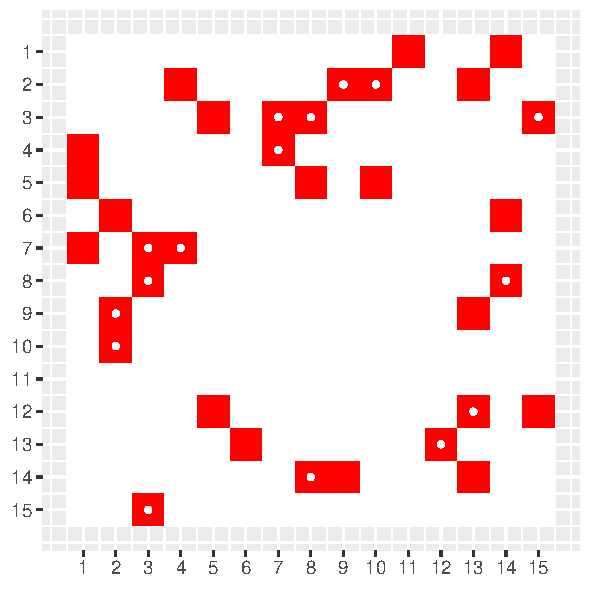
\includegraphics[height=0.8\textheight]{figures/penta-W.pdf}
		\caption{True $\WW$}
	\end{figure}
\end{frame}

\begin{frame}{Basic \acrshort{ergm}: Results P10 $\WW$}
	\begin{figure}[H]
		\centering
		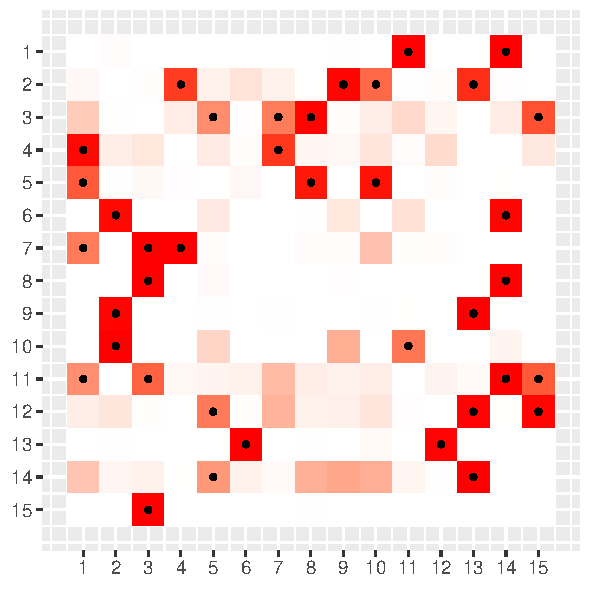
\includegraphics[height=0.8\textheight]{figures/P10-posterior-W.pdf}
		\caption{Posterior Mean $\WW$}
	\end{figure}
\end{frame}

\begin{frame}{Basic \acrshort{ergm}: Results P11 $\WW$}
	\begin{figure}[H]
		\centering
		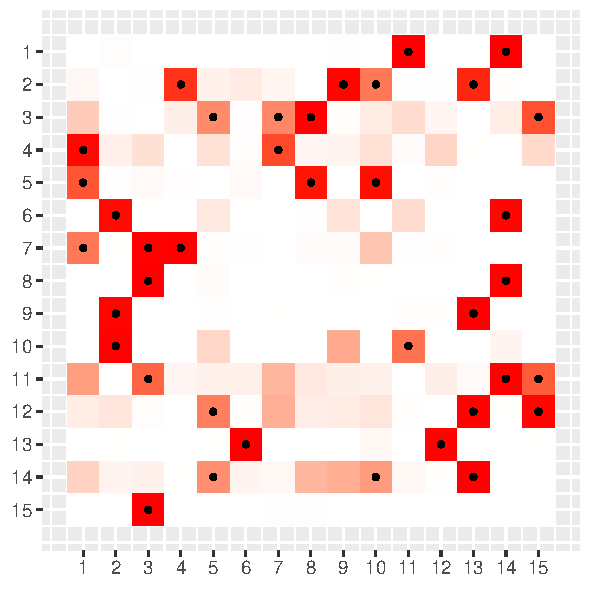
\includegraphics[height=0.8\textheight]{figures/P11-posterior-W.pdf}
		\caption{Posterior Mean $\WW$}
	\end{figure}
\end{frame}

\begin{frame}{Basic \acrshort{ergm}: Results P12 $\WW$}
	\begin{figure}[H]
		\centering
		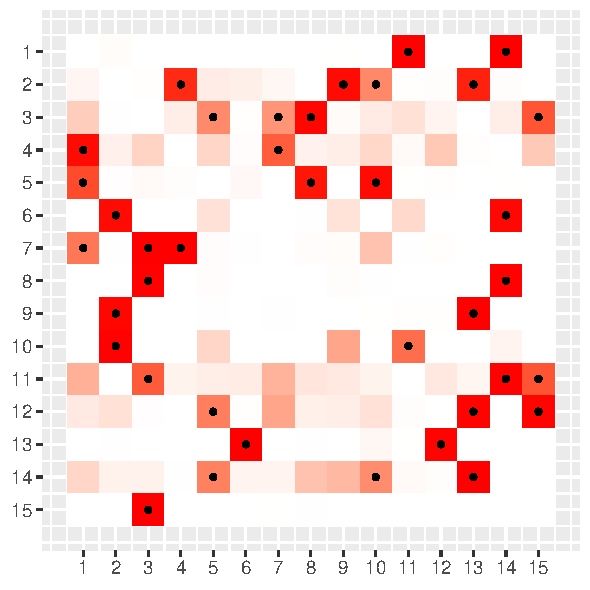
\includegraphics[height=0.8\textheight]{figures/P12-posterior-W.pdf}
		\caption{Posterior Mean $\WW$}
	\end{figure}
\end{frame}

\begin{frame}{Basic \acrshort{ergm}: Results P13 $\WW$}
	\begin{figure}[H]
		\centering
		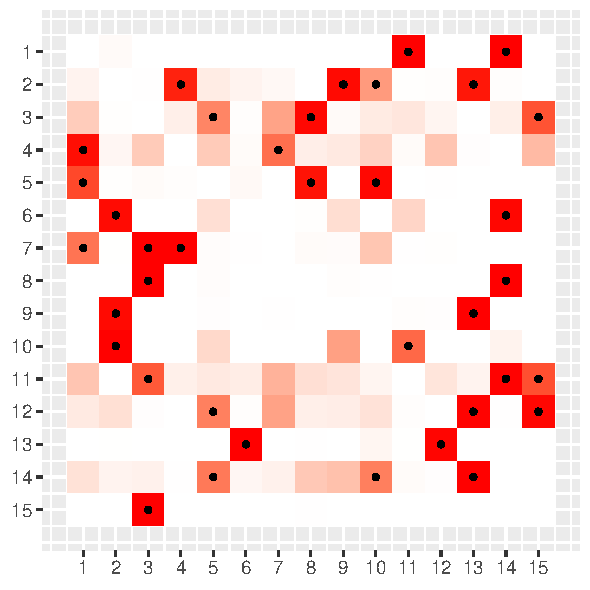
\includegraphics[height=0.8\textheight]{figures/P13-posterior-W.pdf}
		\caption{Posterior Mean $\WW$}
	\end{figure}
\end{frame}

\begin{frame}{Basic \acrshort{ergm}: Results P14 $\WW$}
	\begin{figure}[H]
		\centering
		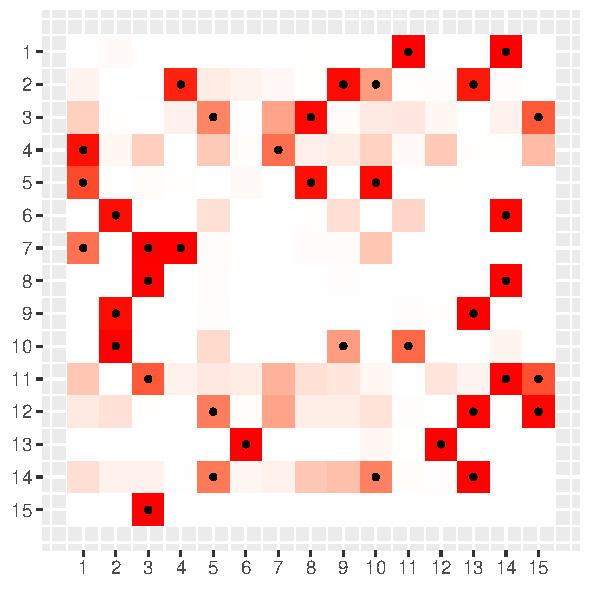
\includegraphics[height=0.8\textheight]{figures/P14-posterior-W.pdf}
		\caption{Posterior Mean $\WW$}
	\end{figure}
\end{frame}

\begin{frame}{Basic \acrshort{ergm}: Results P1}
	\begin{center}
		\footnotesize
		\begin{tabular}{cl|rlrrr}
			\toprule
			\multirow{2}{*}{Spec.} &
			\multirow{2}{*}{Param.} &
			\multirow{2}{*}{True}  &
			\multirow{2}{*}{Prior Dist.} &
			\multirow{2}{*}{Post.\ Mean} &
			\multicolumn{2}{c}{$95\%$ Credible Interval} \\
			& & & & & $Q_{2.5\%}$ & $Q_{97.5\%}$ \\
			\midrule
			\multirow{6}{*}{\shortstack[c]{P12\\$T=12$}}
			& $\lambda$                        & $0.1$ & $\Uniform(-1,1)$       & $0.0323$  & $-0.0355$ & $0.0964$  \\
			& $\sigma^2$                       & $2$   & $\InverseGamma(1,1)$   & $4.5741$  & $3.3396$  & $6.2076$  \\
			& $\bbeta_{1}$                     & $1$   & $\Normal(0,30)$        & $0.9944$  & $0.9584$  & $1.0334$  \\
			& $\bbeta_{2}$                     & $0.5$ & $\Normal(0,30)$        & $0.5930$  & $0.5386$  & $0.6543$  \\
			& $\ttheta_{\text{\Verb"edges"}}$  & $-2$  & $\Normal(0,1)$  & $-1.5410$ & $-2.0779$ & $-1.0458$ \\
			& $\ttheta_{\text{\Verb"mutual"}}$ & $2$   & $\Normal(0,1)$  & $0.4882$  & $-0.6913$ & $1.6313$  \\
			\midrule
			\multirow{5}{*}{\shortstack[c]{P13\\$T=12$}}
			& $\lambda$                        & $0.1$ & $\Uniform(-1,1)$       & $0.0333$  & $-0.0311$ & $0.0991$  \\
			& $\sigma^2$                       & $2$   & $\InverseGamma(1,1)$   & $4.6069$  & $3.3528$  & $6.1911$  \\
			& $\bbeta_{1}$                     & $1$   & $\Normal(0,30)$        & $0.9937$  & $0.9572$  & $1.0308$  \\
			& $\bbeta_{2}$                     & $0.5$ & $\Normal(0,30)$        & $0.5929$  & $0.5382$  & $0.6487$  \\
			& $\ttheta_{\text{\Verb"edges"}}$  & $-2$  & $\Normal(0,1)$  & $-1.4252$ & $-1.8560$ & $-1.0364$ \\
			\bottomrule
		\end{tabular}
	\end{center}
\end{frame}

\begin{frame}{Basic \acrshort{ergm}: Results P20 $\WW$}
	\begin{figure}[H]
		\centering
		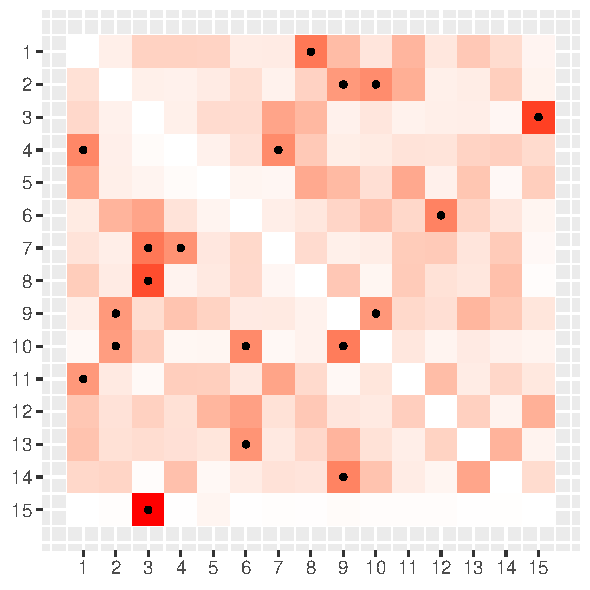
\includegraphics[height=0.8\textheight]{figures/P20-posterior-W.pdf}
		\caption{Posterior Mean $\WW$}
	\end{figure}
\end{frame}

\begin{frame}{Basic \acrshort{ergm}: Results P21 $\WW$}
	\begin{figure}[H]
		\centering
		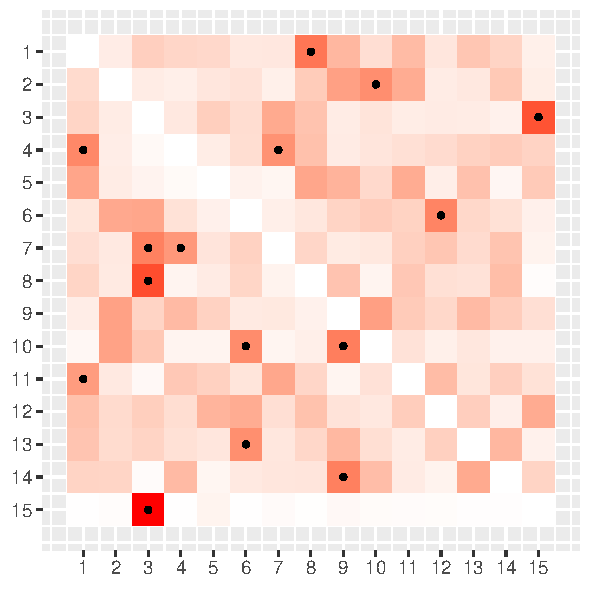
\includegraphics[height=0.8\textheight]{figures/P21-posterior-W.pdf}
		\caption{Posterior Mean $\WW$}
	\end{figure}
\end{frame}

\begin{frame}{Basic \acrshort{ergm}: Results P22 $\WW$}
	\begin{figure}[H]
		\centering
		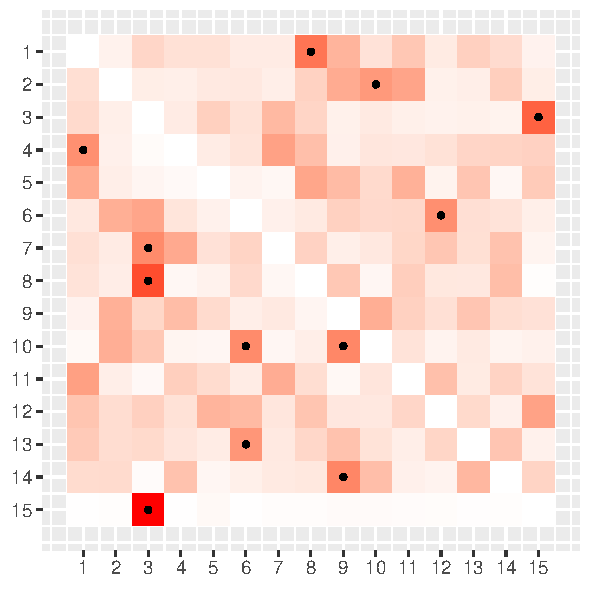
\includegraphics[height=0.8\textheight]{figures/P22-posterior-W.pdf}
		\caption{Posterior Mean $\WW$}
	\end{figure}
\end{frame}

\begin{frame}{Basic \acrshort{ergm}: Results P23 $\WW$}
	\begin{figure}[H]
		\centering
		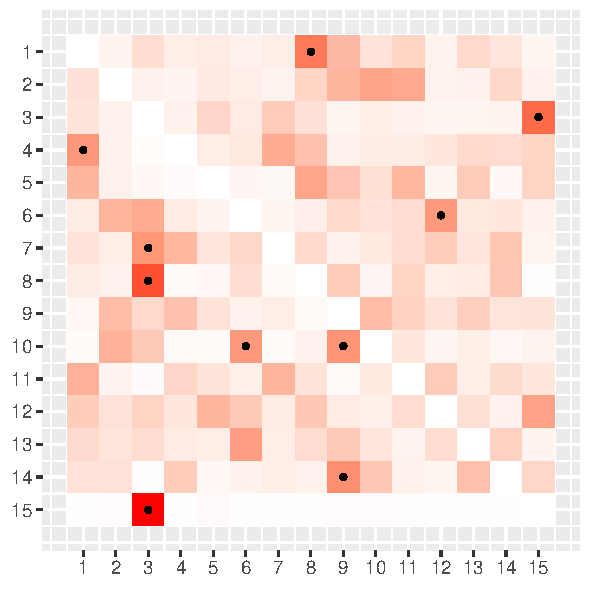
\includegraphics[height=0.8\textheight]{figures/P23-posterior-W.pdf}
		\caption{Posterior Mean $\WW$}
	\end{figure}
\end{frame}

\begin{frame}{Basic \acrshort{ergm}: Results P24 $\WW$}
	\begin{figure}[H]
		\centering
		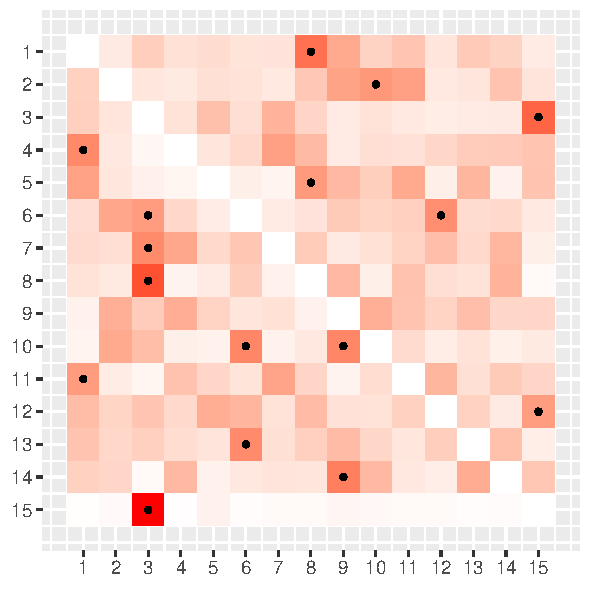
\includegraphics[height=0.8\textheight]{figures/P24-posterior-W.pdf}
		\caption{Posterior Mean $\WW$}
	\end{figure}
\end{frame}

\begin{frame}{Basic \acrshort{ergm}: Results P2}
	\begin{center}
		\footnotesize
		\begin{tabular}{cl|rlrrr}
			\toprule
			\multirow{2}{*}{Spec.} &
			\multirow{2}{*}{Param.} &
			\multirow{2}{*}{True}  &
			\multirow{2}{*}{Prior Dist.} &
			\multirow{2}{*}{Post.\ Mean} &
			\multicolumn{2}{c}{$95\%$ Credible Interval} \\
			& & & & & $Q_{2.5\%}$ & $Q_{97.5\%}$ \\
			\midrule
			\multirow{6}{*}{\shortstack[c]{P22\\$T=12$}}
			& $\lambda$                        & $0.1$ & $\Uniform(-1,1)$       & $0.0978$  & $0.0470$  & $0.1466$  \\
			& $\sigma^2$                       & $2$   & $\InverseGamma(1,1)$   & $2.2190$  & $1.6317$  & $3.1347$  \\
			& $\bbeta_{1}$                     & $1$   & $\Normal(0,30)$        & $1.0026$  & $0.9795$  & $1.0253$  \\
			& $\bbeta_{2}$                     & $0.5$ & $\Normal(0,30)$        & $0.1891$  & $0.1736$  & $0.2049$  \\
			& $\ttheta_{\text{\Verb"edges"}}$  & $-2$  & $\Normal(0,1)$  & $-1.7877$ & $-3.4018$ & $-0.7241$ \\
			& $\ttheta_{\text{\Verb"mutual"}}$ & $2$   & $\Normal(0,1)$  & $0.2623$  & $-1.3760$ & $1.7652$  \\
			\midrule
			\multirow{5}{*}{\shortstack[c]{P23\\$T=12$}}
			& $\lambda$                        & $0.1$ & $\Uniform(-1,1)$       & $0.0930$  & $0.0454$  & $0.1403$  \\
			& $\sigma^2$                       & $2$   & $\InverseGamma(1,1)$   & $2.2601$  & $1.6619$  & $3.2626$  \\
			& $\bbeta_{1}$                     & $1$   & $\Normal(0,30)$        & $1.0042$  & $0.9813$  & $1.0287$  \\
			& $\bbeta_{2}$                     & $0.5$ & $\Normal(0,30)$        & $0.1894$  & $0.1735$  & $0.2056$  \\
			& $\ttheta_{\text{\Verb"edges"}}$  & $-2$  & $\Normal(0,1)$  & $-1.9940$ & $-4.0807$ & $-0.8732$ \\
			\bottomrule
		\end{tabular}
	\end{center}
\end{frame}

\begin{frame}{Basic \acrshort{ergm}: Results Summary}
	\begin{itemize}
		\item
			Significant results are obtained for $\lambda$,
			however, this depends heavily on the model specification.
			\begin{itemize}
				\item In general, $\pr(\lambda\given\WW,\{\yy_{t}\})$ is very different from $\pr(\lambda,\WW\given\{\yy_{t}\})$
			\end{itemize}
		\item
			The spatial matrix $\WW$ is well-recovered by the approach.
		\item
			Inference of $\ttheta$ is as expected,
			but only \texttt{edges} obtain consistently significant results.
		\item
			Our model out performs specifications where only $\ttheta_{\text{\Verb"edges"}}$ is specified in the prior,
			but only by a little.
	\end{itemize}
\end{frame}

\subsection{Sampson's Monk}

\begin{frame}[fragile]{Sampson's Monk}
	\begin{center}
		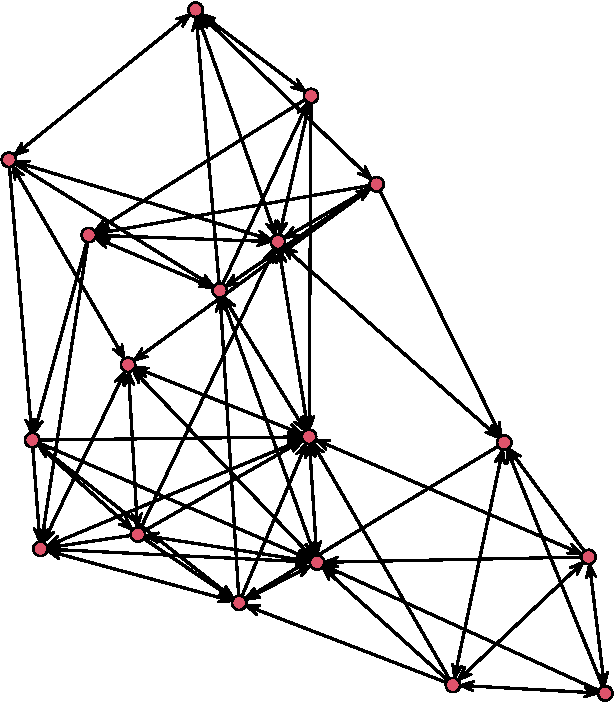
\includegraphics[width=0.40\textwidth]{figures/sampson.pdf}
		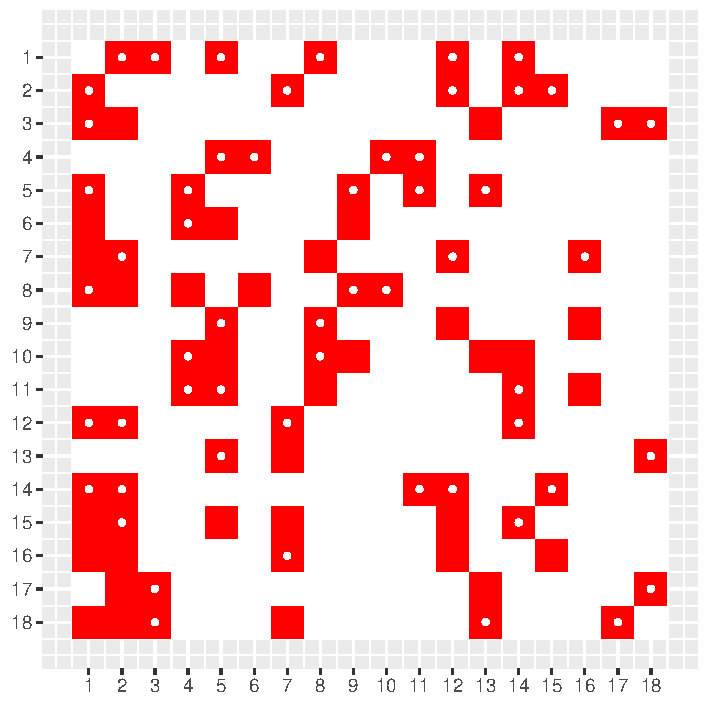
\includegraphics[width=0.45\textwidth]{figures/sampson-W.pdf}
	\end{center}
	\begin{itemize}
		\item
			We use \acrshort{ergm} with
			$\text{\Verb"edges"}=-3$,
			$\text{\Verb"mutual"}=2$, and
			$\text{\Verb"ctriad"}=-0.5$ as prior.
	\end{itemize}
\end{frame}

\begin{frame}{Group S1 and S2}
	\begin{enumerate}
		\item\blue{\textbf{Group S1}}:
			$\XX_1=\XX_2$ are $N\times 2$ matrix of exogenous variables.
			In this group, the exogenous effects are larger than endogenous effects.
		\item\blue{\textbf{Group S2}}:
			$\XX_1=\XX_2$ are $N\times 2$ matrix of exogenous variables.
			In this group, the some exogenous effects are smaller than some endogenous effects.
	\end{enumerate}
\end{frame}

\begin{frame}{Sampson's Monk: Results}
	\begin{figure}[H]
		\centering
		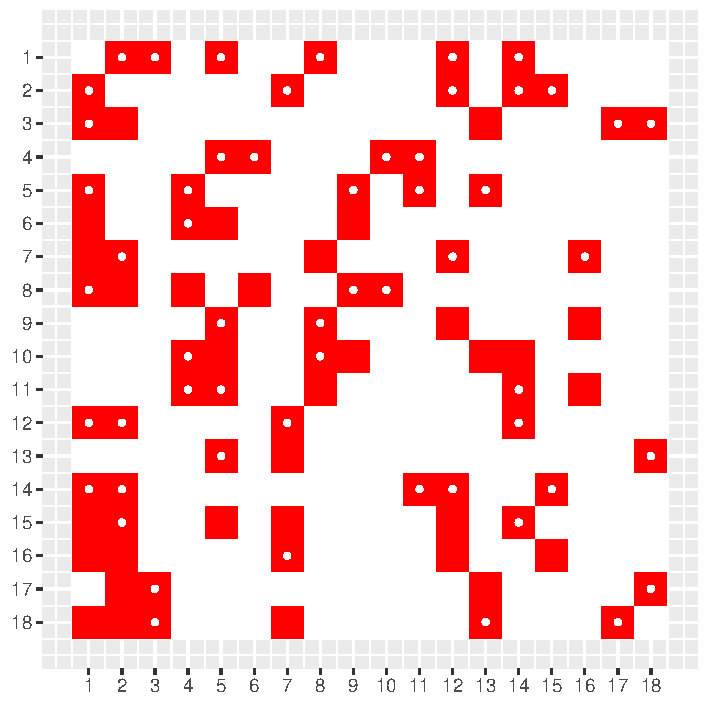
\includegraphics[height=0.8\textheight]{figures/sampson-W.pdf}
		\caption{True $\WW$}
	\end{figure}
\end{frame}

\begin{frame}{Sampson's Monk: Results S10 $\WW$}
	\begin{figure}[H]
		\centering
		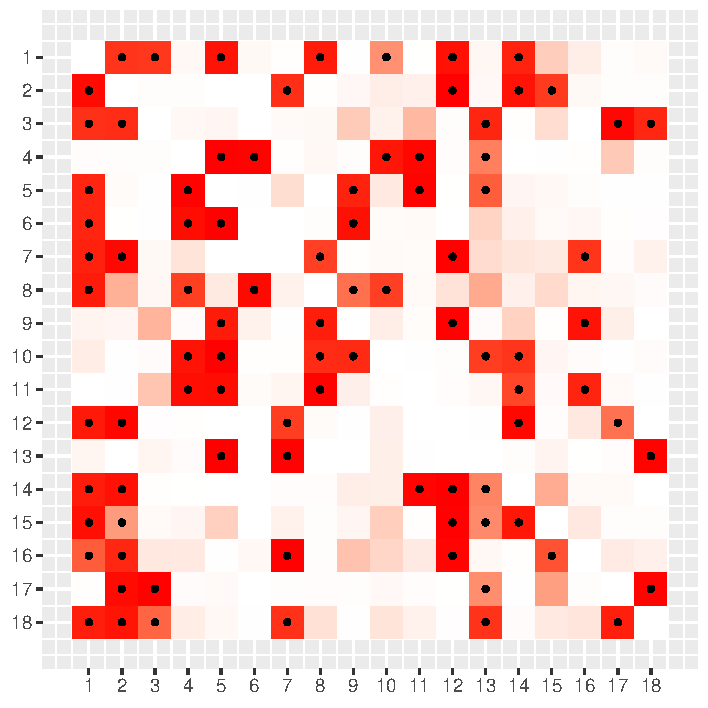
\includegraphics[height=0.8\textheight]{figures/S10-posterior-W.pdf}
		\caption{Posterior Mean $\WW$}
	\end{figure}
\end{frame}

\begin{frame}{Sampson's Monk: Results S11 $\WW$}
	\begin{figure}[H]
		\centering
		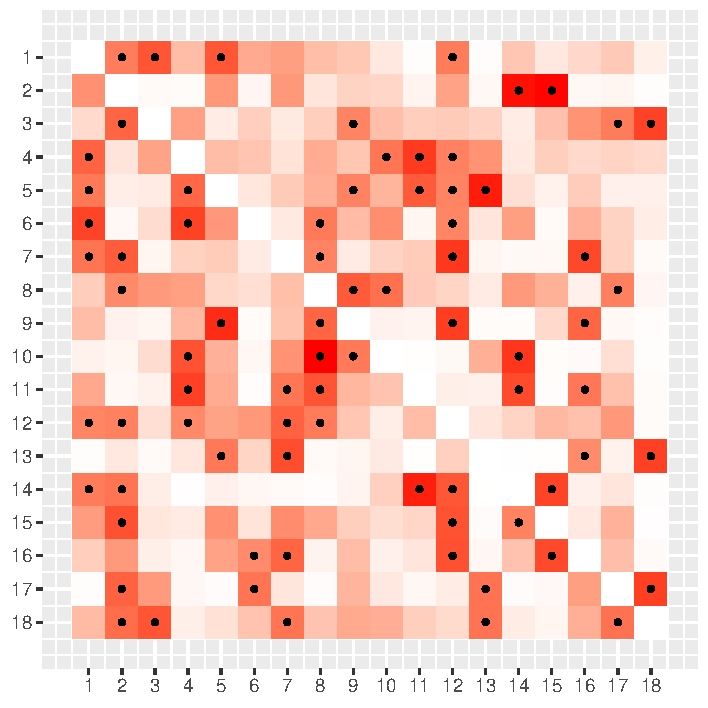
\includegraphics[height=0.8\textheight]{figures/S11-posterior-W.pdf}
		\caption{Posterior Mean $\WW$}
	\end{figure}
\end{frame}

\begin{frame}{Sampson's Monk: Results S12 $\WW$}
	\begin{figure}[H]
		\centering
		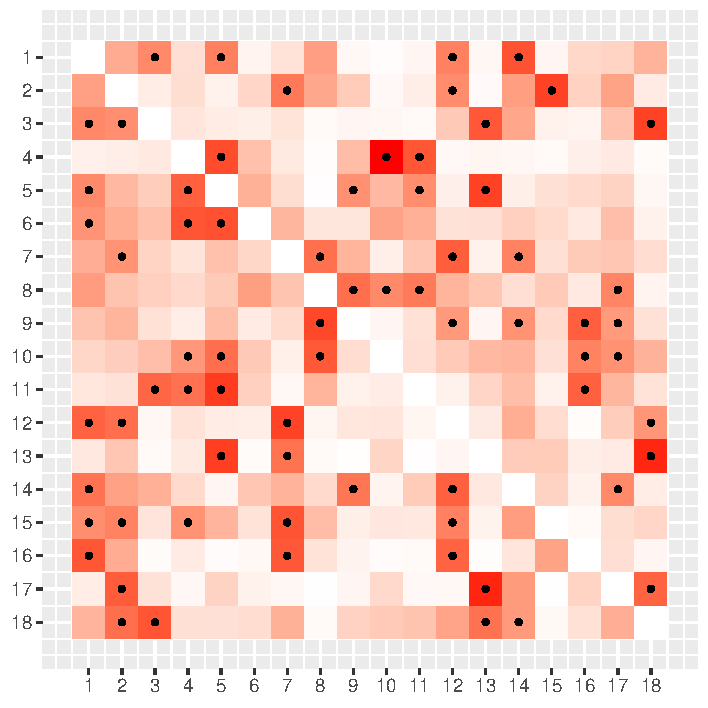
\includegraphics[height=0.8\textheight]{figures/S12-posterior-W.pdf}
		\caption{Posterior Mean $\WW$}
	\end{figure}
\end{frame}

\begin{frame}{Sampson's Monk: Results S1}
	\begin{center}
		\scriptsize
		\begin{tabular}{cl|rlrrr}
			\toprule
			\multirow{2}{*}{Spec.} &
			\multirow{2}{*}{Param.} &
			\multirow{2}{*}{True}  &
			\multirow{2}{*}{Prior Dist.} &
			\multirow{2}{*}{Post.\ Mean} &
			\multicolumn{2}{c}{$95\%$ Credible Interval} \\
			& & & & & $Q_{2.5\%}$ & $Q_{97.5\%}$ \\
			\midrule
			\multirow{9}{*}{\shortstack[c]{S10\\$T=18$}}
			& $\lambda$                        & $0.1$  & $\Uniform(-1,1)$     & $0.0320$  & $-0.0857$ & $0.1964$  \\
			& $\sigma^2$                       & $2$    & $\InverseGamma(1,1)$ & $2.8549$  & $1.9332$  & $5.6295$  \\
			& $\bbeta_{1,1}$                   & $2$    & $\Normal(0,30)$      & $2.0123$  & $1.9648$  & $2.0617$  \\
			& $\bbeta_{1,2}$                   & $2$    & $\Normal(0,30)$      & $2.0984$  & $1.1329$  & $2.7002$  \\
			& $\bbeta_{2,1}$                   & $0.5$  & $\Normal(0,30)$      & $0.7005$  & $0.4930$  & $0.8812$  \\
			& $\bbeta_{2,2}$                   & $0.5$  & $\Normal(0,30)$      & $0.1332$  & $-5.8634$ & $3.3570$  \\
			& $\ttheta_{\text{\Verb"edges"}}$  & $-1.8$ & $\Normal(-3,1)$      & $-0.9080$ & $-1.6285$ & $-0.0488$ \\
			& $\ttheta_{\text{\Verb"mutual"}}$ & $2.3$  & $\Normal(2,1)$       & $1.2242$  & $0.3165$  & $2.1608$  \\
			& $\ttheta_{\text{\Verb"ctriad"}}$ & $-0.1$ & $\Normal(-0.5,1)$    & $-0.2491$ & $-0.7051$ & $0.1311$  \\
			\midrule
			\multirow{9}{*}{\shortstack[c]{S11\\$T=12$}}
			& $\lambda$                        & $0.1$  & $\Uniform(-1,1)$     & $0.0306$  & $-0.0906$  & $0.1989$  \\
			& $\sigma^2$                       & $2$    & $\InverseGamma(1,1)$ & $4.6437$  & $1.7827$   & $11.3241$ \\
			& $\bbeta_{1,1}$                   & $2$    & $\Normal(0,30)$      & $2.0015$  & $1.9525$   & $2.0572$  \\
			& $\bbeta_{1,2}$                   & $2$    & $\Normal(0,30)$      & $4.2848$  & $1.2563$   & $10.8403$ \\
			& $\bbeta_{2,1}$                   & $0.5$  & $\Normal(0,30)$      & $0.6090$  & $0.0223$   & $0.9359$  \\
			& $\bbeta_{2,2}$                   & $0.5$  & $\Normal(0,30)$      & $0.9627$  & $-12.6832$ & $10.0607$ \\
			& $\ttheta_{\text{\Verb"edges"}}$  & $-1.8$ & $\Normal(-3,1)$      & $-1.2569$ & $-4.7459$  & $0.3174$  \\
			& $\ttheta_{\text{\Verb"mutual"}}$ & $2.3$  & $\Normal(2,1)$       & $0.6115$  & $-1.0884$  & $1.8689$  \\
			& $\ttheta_{\text{\Verb"ctriad"}}$ & $-0.1$ & $\Normal(-0.5,1)$    & $-0.3708$ & $-1.9857$  & $0.2509$  \\
			\bottomrule
		\end{tabular}
	\end{center}
\end{frame}

\begin{frame}{Sampson's Monk: Results S20 $\WW$}
	\begin{figure}[H]
		\centering
		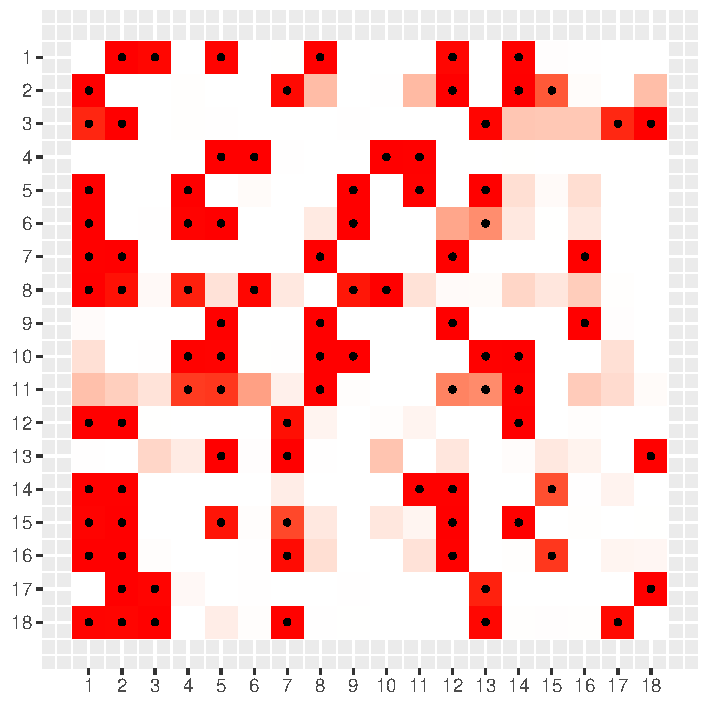
\includegraphics[height=0.8\textheight]{figures/S20-posterior-W.pdf}
		\caption{Posterior Mean $\WW$}
	\end{figure}
\end{frame}

\begin{frame}{Sampson's Monk: Results S21 $\WW$}
	\begin{figure}[H]
		\centering
		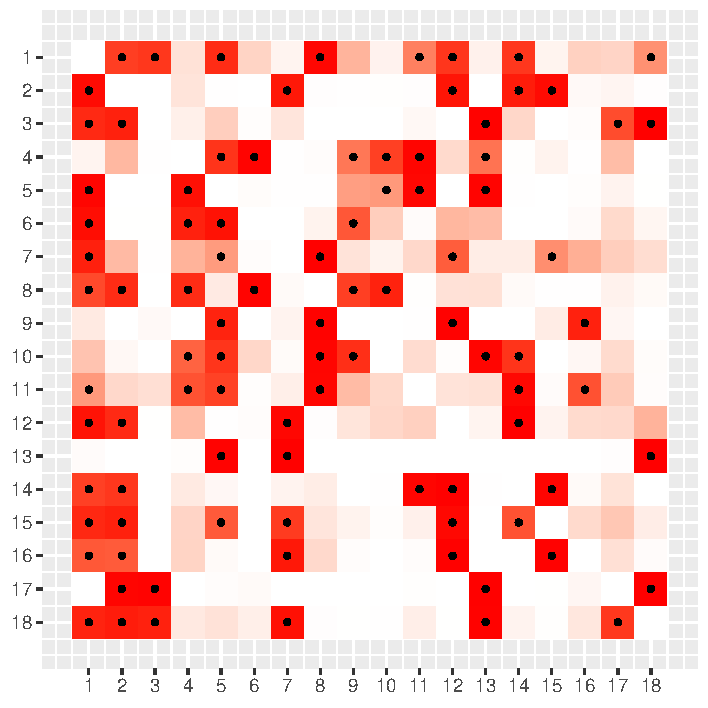
\includegraphics[height=0.8\textheight]{figures/S21-posterior-W.pdf}
		\caption{Posterior Mean $\WW$}
	\end{figure}
\end{frame}

\begin{frame}{Sampson's Monk: Results S22 $\WW$}
	\begin{figure}[H]
		\centering
		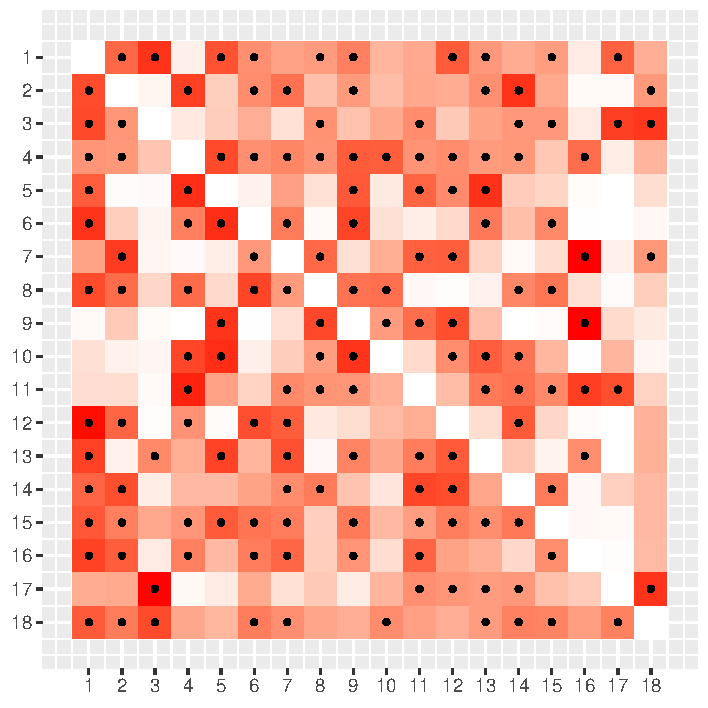
\includegraphics[height=0.8\textheight]{figures/S22-posterior-W.pdf}
		\caption{Posterior Mean $\WW$}
	\end{figure}
\end{frame}

\begin{frame}{Sampson's Monk: Results S2}
	\begin{center}
		\scriptsize
		\begin{tabular}{cl|rlrrr}
			\toprule
			\multirow{2}{*}{Spec.} &
			\multirow{2}{*}{Param.} &
			\multirow{2}{*}{True}  &
			\multirow{2}{*}{Prior Dist.} &
			\multirow{2}{*}{Post.\ Mean} &
			\multicolumn{2}{c}{$95\%$ Credible Interval} \\
			& & & & & $Q_{2.5\%}$ & $Q_{97.5\%}$ \\
			\midrule
			\multirow{9}{*}{\shortstack[c]{S20\\$T=18$}}
			& $\lambda$                        & $0.1$  & $\Uniform(-1,1)$     & $0.0933$  & $-0.0515$ & $0.2552$  \\
			& $\sigma^2$                       & $2$    & $\InverseGamma(1,1)$ & $6.0217$  & $3.3168$  & $10.7843$ \\
			& $\bbeta_{1,1}$                   & $2$    & $\Normal(0,30)$      & $1.9934$  & $1.9176$  & $2.0710$  \\
			& $\bbeta_{1,2}$                   & $0.5$  & $\Normal(0,30)$      & $0.8951$  & $-0.1525$ & $1.8155$  \\
			& $\bbeta_{2,1}$                   & $2$    & $\Normal(0,30)$      & $2.0583$  & $1.5653$  & $2.4986$  \\
			& $\bbeta_{2,2}$                   & $0.5$  & $\Normal(0,30)$      & $-0.7854$ & $-5.3961$ & $3.1025$  \\
			& $\ttheta_{\text{\Verb"edges"}}$  & $-1.8$ & $\Normal(-3,1)$      & $-1.2451$ & $-1.8671$ & $-0.5679$ \\
			& $\ttheta_{\text{\Verb"mutual"}}$ & $2.3$  & $\Normal(2,1)$       & $1.0436$  & $0.1724$  & $1.9152$  \\
			& $\ttheta_{\text{\Verb"ctriad"}}$ & $-0.1$ & $\Normal(-0.5,1)$    & $0.0069$  & $-0.3277$ & $0.2604$  \\
			\midrule
			\multirow{9}{*}{\shortstack[c]{S21\\$T=12$}}
			& $\lambda$                        & $0.1$  & $\Uniform(-1,1)$     & $0.0339$  & $-0.1151$ & $0.2276$  \\
			& $\sigma^2$                       & $2$    & $\InverseGamma(1,1)$ & $6.1242$  & $3.2807$  & $13.9441$ \\
			& $\bbeta_{1,1}$                   & $2$    & $\Normal(0,30)$      & $2.0333$  & $1.8949$  & $2.1770$  \\
			& $\bbeta_{1,2}$                   & $0.5$  & $\Normal(0,30)$      & $0.9477$  & $-0.1826$ & $2.3512$  \\
			& $\bbeta_{2,1}$                   & $2$    & $\Normal(0,30)$      & $2.2310$  & $1.7853$  & $2.5866$  \\
			& $\bbeta_{2,2}$                   & $0.5$  & $\Normal(0,30)$      & $1.4372$  & $-3.9601$ & $5.0759$  \\
			& $\ttheta_{\text{\Verb"edges"}}$  & $-1.8$ & $\Normal(-3,1)$      & $-1.1667$ & $-1.7794$ & $-0.5208$ \\
			& $\ttheta_{\text{\Verb"mutual"}}$ & $2.3$  & $\Normal(2,1)$       & $0.8031$  & $-0.0575$ & $1.6794$  \\
			& $\ttheta_{\text{\Verb"ctriad"}}$ & $-0.1$ & $\Normal(-0.5,1)$    & $0.0580$  & $-0.2533$ & $0.2849$  \\
			\bottomrule
		\end{tabular}
	\end{center}
\end{frame}

\begin{frame}{Sampson's Monk: Results Summary}
	\begin{itemize}
		\item
			The posterior $\WW$ is more noisy when the network is more busy.
		\item
			Similar to the first simulation study, no significant result for $\lambda$.
		\item
			Posterior inferences for $\ttheta$ is as expected:
			more significant results when the panel is longer.
		\item
			Matrix degeneracy is a problem in this simulation.
	\end{itemize}
\end{frame}

\subsection{Zachary's Karate Cub}

\begin{frame}{Zachary's Karate Cub}
	\begin{center}
		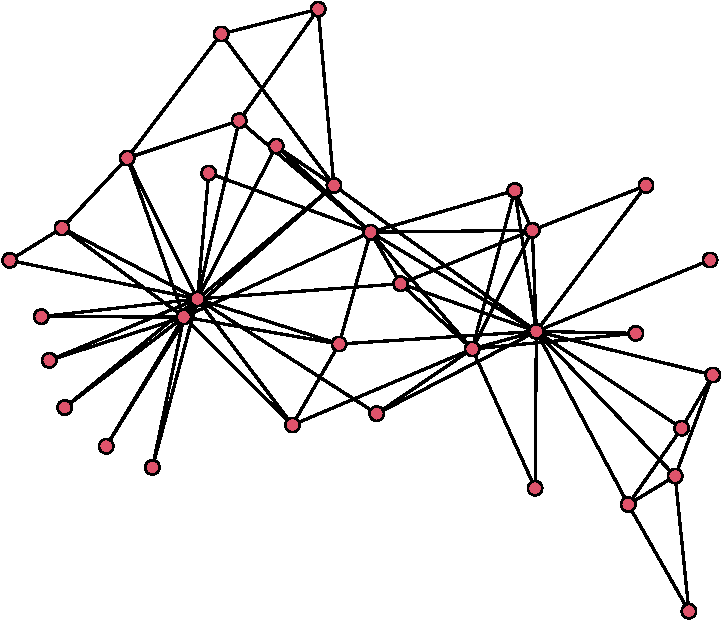
\includegraphics[width=0.50\textwidth]{figures/zach.pdf}
		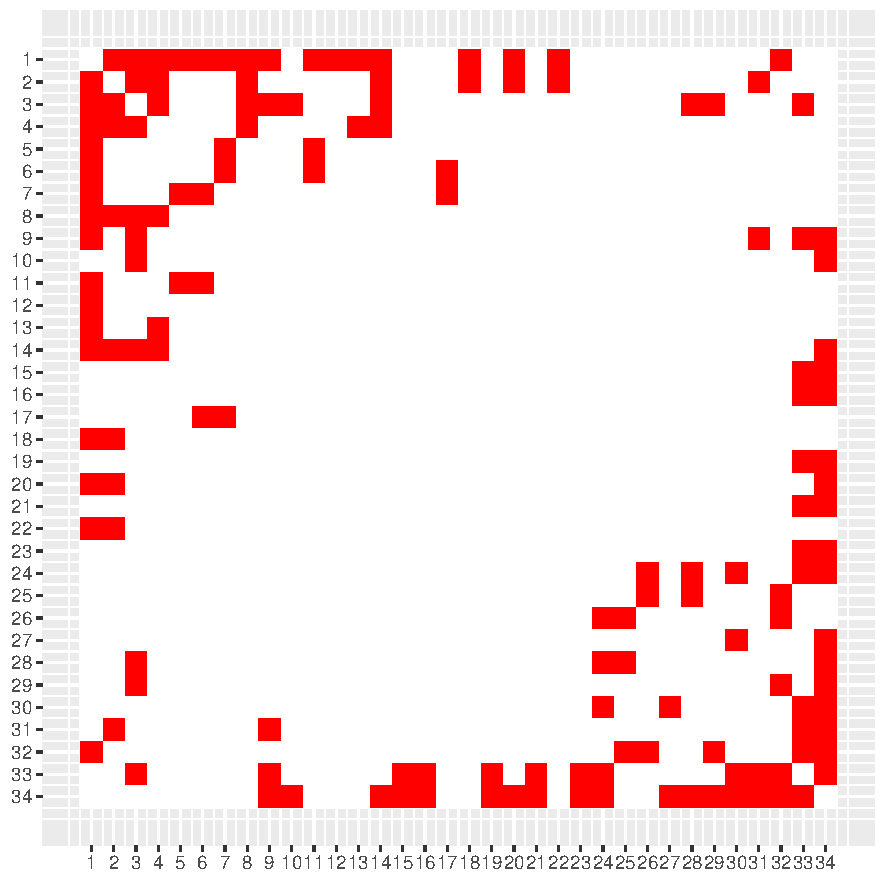
\includegraphics[width=0.45\textwidth]{figures/zach-W.pdf}
	\end{center}
	\begin{itemize}
		\item
			For this undirected network,
			we use \acrshort{ergm} with
			$\text{\Verb"edges"}=-2$,
			$\text{\Verb"2-star"}=0.2$,
			$\text{\Verb"3-star"}=-0.1$, and
			$\text{\Verb"triangle"}=0.3$.
	\end{itemize}
\end{frame}

\begin{frame}{Group K1 and K2}
	\begin{itemize}
		\item\blue{\textbf{Group K1}}:
			$\XX_1$ is an $N\times 2$ matrix of exogenous variables.
			The endogenous effect of this group is $\lambda=0.05$.
		\item\blue{\textbf{Group K2}}:
			$\XX_1$ is an $N\times 2$ matrix of exogenous variables.
			The endogenous effect of this group is $\lambda=0.1$.
	\end{itemize}
\end{frame}

\begin{frame}{Zachary's Karate Club: Results}
	\begin{figure}[H]
		\centering
		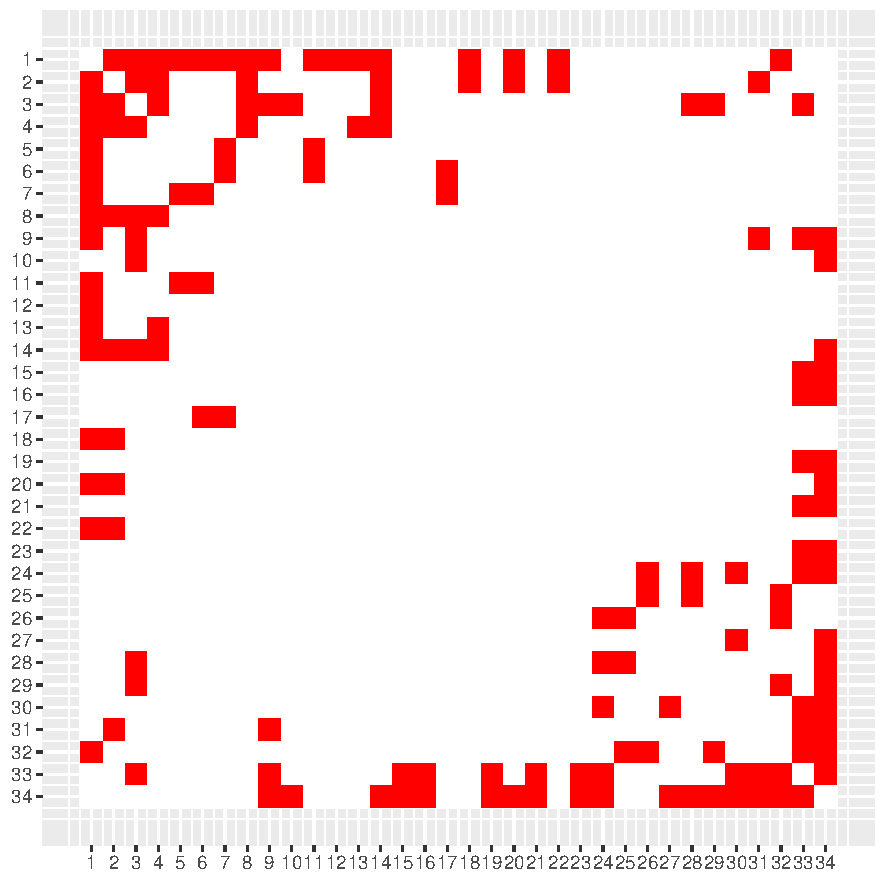
\includegraphics[height=0.8\textheight]{figures/zach-W.pdf}
		\caption{True $\WW$}
	\end{figure}
\end{frame}

\begin{frame}{Zachary's Karate Club: Results K10 $\WW$}
	\begin{figure}[H]
		\centering
		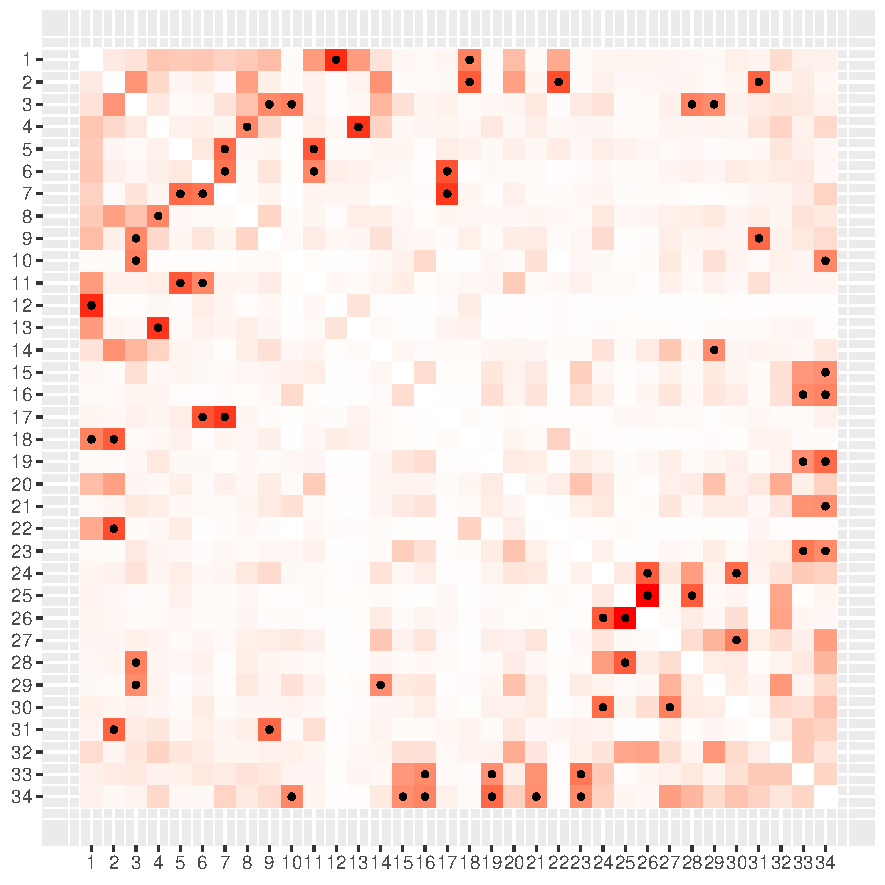
\includegraphics[height=0.8\textheight]{figures/K10-posterior-W.pdf}
		\caption{Posterior Mean $\WW$}
	\end{figure}
\end{frame}

\begin{frame}{Zachary's Karate Club: Results K11 $\WW$}
	\begin{figure}[H]
		\centering
		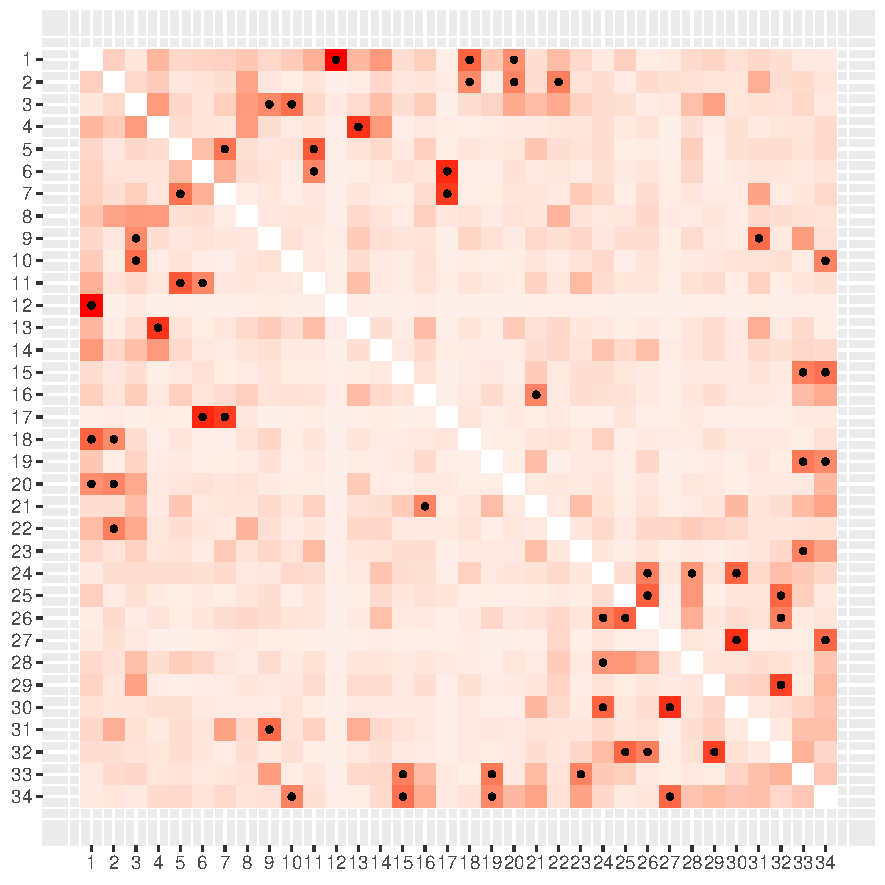
\includegraphics[height=0.8\textheight]{figures/K11-posterior-W.pdf}
		\caption{Posterior Mean $\WW$}
	\end{figure}
\end{frame}

\begin{frame}{Zachary's Karate Club: Results K12 $\WW$}
	\begin{figure}[H]
		\centering
		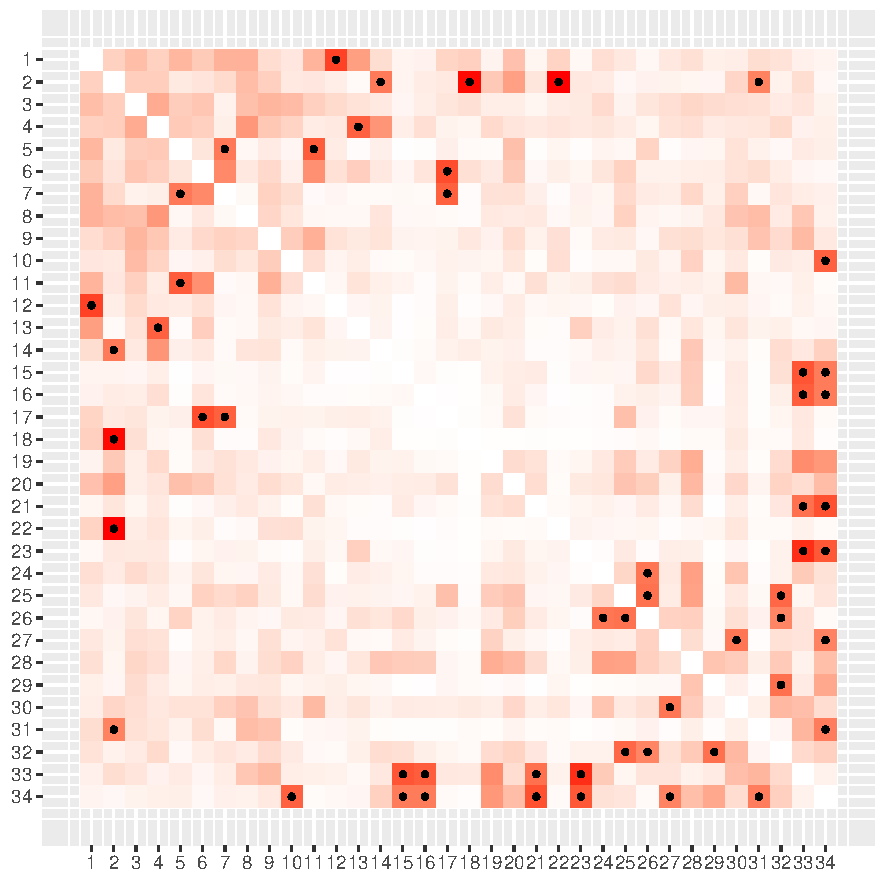
\includegraphics[height=0.8\textheight]{figures/K12-posterior-W.pdf}
		\caption{Posterior Mean $\WW$}
	\end{figure}
\end{frame}

\begin{frame}{Zachary's Karate Club: Results K1} %
	\begin{center}
		\scriptsize
		\begin{tabular}{cl|rlrrr}
			\toprule
			\multirow{2}{*}{Spec.} &
			\multirow{2}{*}{Param.} &
			\multirow{2}{*}{True}  &
			\multirow{2}{*}{Prior Dist.} &
			\multirow{2}{*}{Post.\ Mean} &
			\multicolumn{2}{c}{$95\%$ Credible Interval} \\
			& & & & & $Q_{2.5\%}$ & $Q_{97.5\%}$ \\
			\midrule
			\multirow{9}{*}{\shortstack[c]{K10\\$T=15$}}
			& $\lambda$                          & $0.05$ & $\Uniform(-1,1)$     & $0.2761$  & $-0.3237$  & $0.9442$   \\
			& $\sigma^2$                         & $5$    & $\InverseGamma(1,1)$ & $40.1132$ & $8.4908$   & $173.1849$ \\
			& $\bbeta_{1,1}$                     & $2$    & $\Normal(0,30)$      & $2.0150$  & $1.7000$   & $2.2317$   \\
			& $\bbeta_{1,2}$                     & $1$    & $\Normal(0,30)$      & $0.2775$  & $-10.1314$ & $8.5981$   \\
			& $\bbeta_{2}$                       & $0.5$  & $\Normal(0,30)$      & $-0.1082$ & $-1.7671$  & $1.3477$   \\
			& $\ttheta_{\text{\Verb"edges"}}$    & $-3$   & $\Normal(-3,1)$      & $-2.3436$ & $-3.3285$  & $-1.1674$  \\
			& $\ttheta_{\text{\Verb"2-star"}}$   & $0.2$  & $\Normal(0.2,1)$     & $0.7999$  & $0.1206$   & $1.5804$   \\
			& $\ttheta_{\text{\Verb"3-star"}}$   & $-0.1$ & $\Normal(-0.1,1)$    & $-0.4000$ & $-1.1722$  & $-0.0340$  \\
			& $\ttheta_{\text{\Verb"triangle"}}$ & $0.3$  & $\Normal(0.3,1)$     & $0.2646$  & $-0.8123$  & $1.2890$   \\
			\midrule
			\multirow{9}{*}{\shortstack[c]{K11\\$T=12$}}
			& $\lambda$                          & $0.05$ & $\Uniform(-1,1)$     & $0.0292$  & $-0.3401$ & $0.4165$   \\
			& $\sigma^2$                         & $5$    & $\InverseGamma(1,1)$ & $37.3011$ & $8.3389$  & $149.4285$ \\
			& $\bbeta_{1,1}$                     & $2$    & $\Normal(0,30)$      & $2.0682$  & $1.8333$  & $2.4211$   \\
			& $\bbeta_{1,2}$                     & $1$    & $\Normal(0,30)$      & $1.0926$  & $-4.0489$ & $7.2829$   \\
			& $\bbeta_{2}$                       & $0.5$  & $\Normal(0,30)$      & $0.4879$  & $-0.4604$ & $1.3605$   \\
			& $\ttheta_{\text{\Verb"edges"}}$    & $-3$   & $\Normal(-3,1)$      & $-2.4652$ & $-3.6032$ & $-1.2811$  \\
			& $\ttheta_{\text{\Verb"2-star"}}$   & $0.2$  & $\Normal(0.2,1)$     & $0.7811$  & $-0.0684$ & $1.5686$   \\
			& $\ttheta_{\text{\Verb"3-star"}}$   & $-0.1$ & $\Normal(-0.1,1)$    & $-0.2669$ & $-1.0970$ & $1.1224$   \\
			& $\ttheta_{\text{\Verb"triangle"}}$ & $0.3$  & $\Normal(0.3,1)$     & $0.2900$  & $-0.8121$ & $1.4029$   \\
			\bottomrule
		\end{tabular}
	\end{center}
\end{frame}

\begin{frame}{Zachary's Karate Club: Results K20 $\WW$}
	\begin{figure}[H]
		\centering
		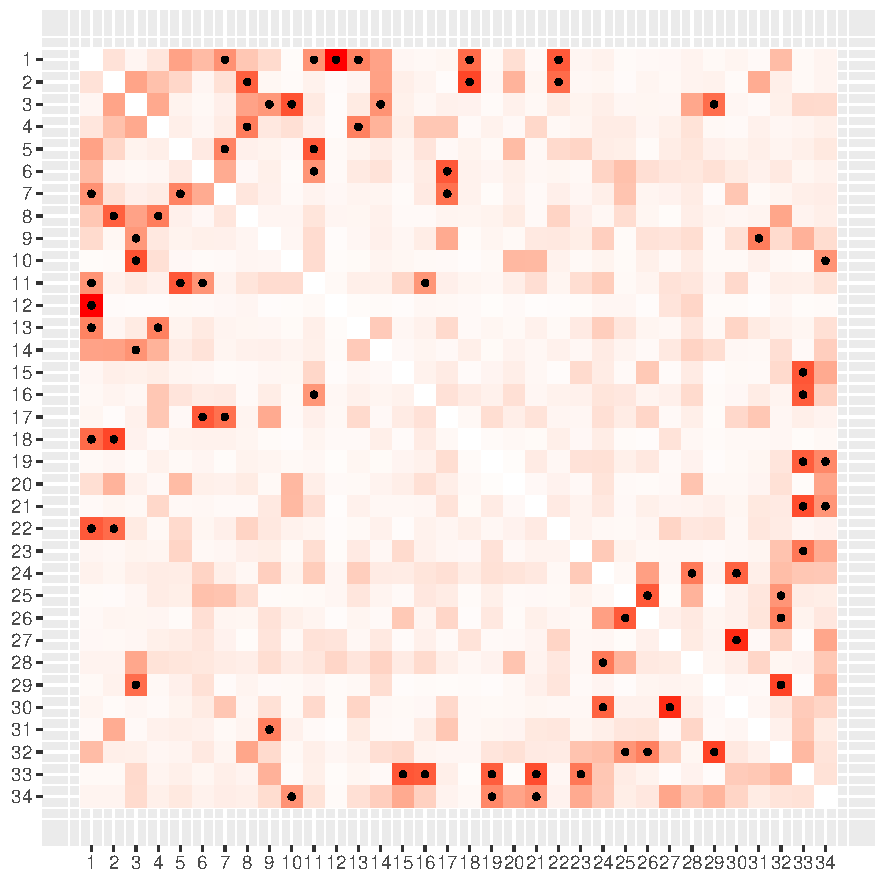
\includegraphics[height=0.8\textheight]{figures/K20-posterior-W.pdf}
		\caption{Posterior Mean $\WW$}
	\end{figure}
\end{frame}

\begin{frame}{Zachary's Karate Club: Results K21 $\WW$}
	\begin{figure}[H]
		\centering
		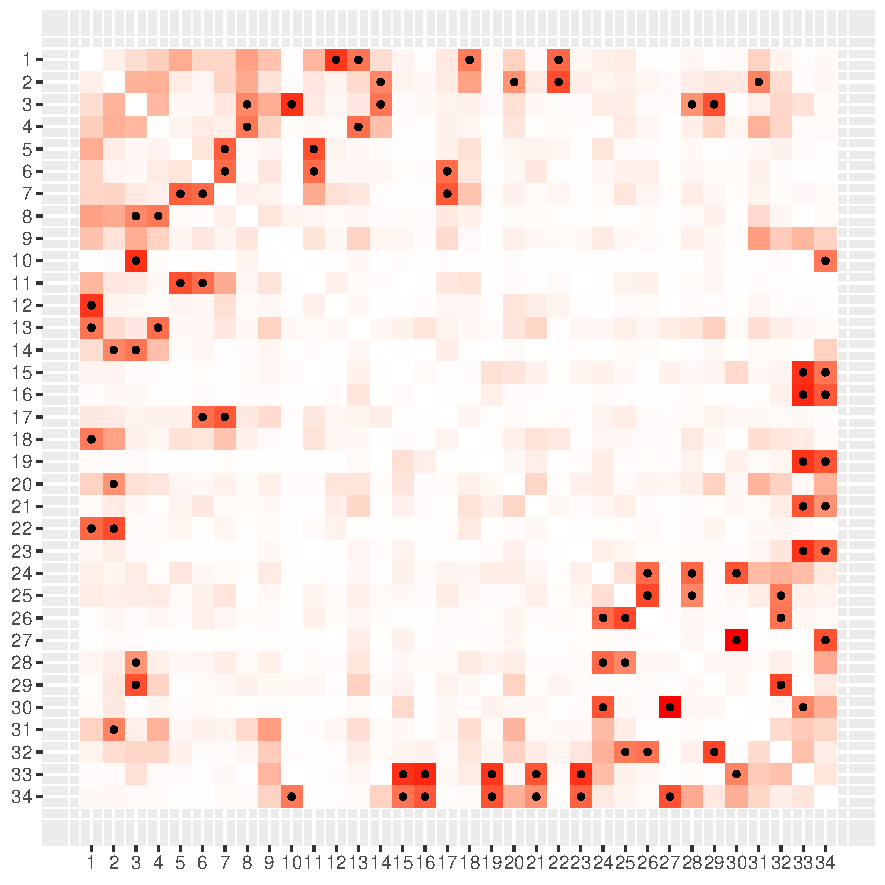
\includegraphics[height=0.8\textheight]{figures/K21-posterior-W.pdf}
		\caption{Posterior Mean $\WW$}
	\end{figure}
\end{frame}

\begin{frame}{Zachary's Karate Club: Results K22 $\WW$}
	\begin{figure}[H]
		\centering
		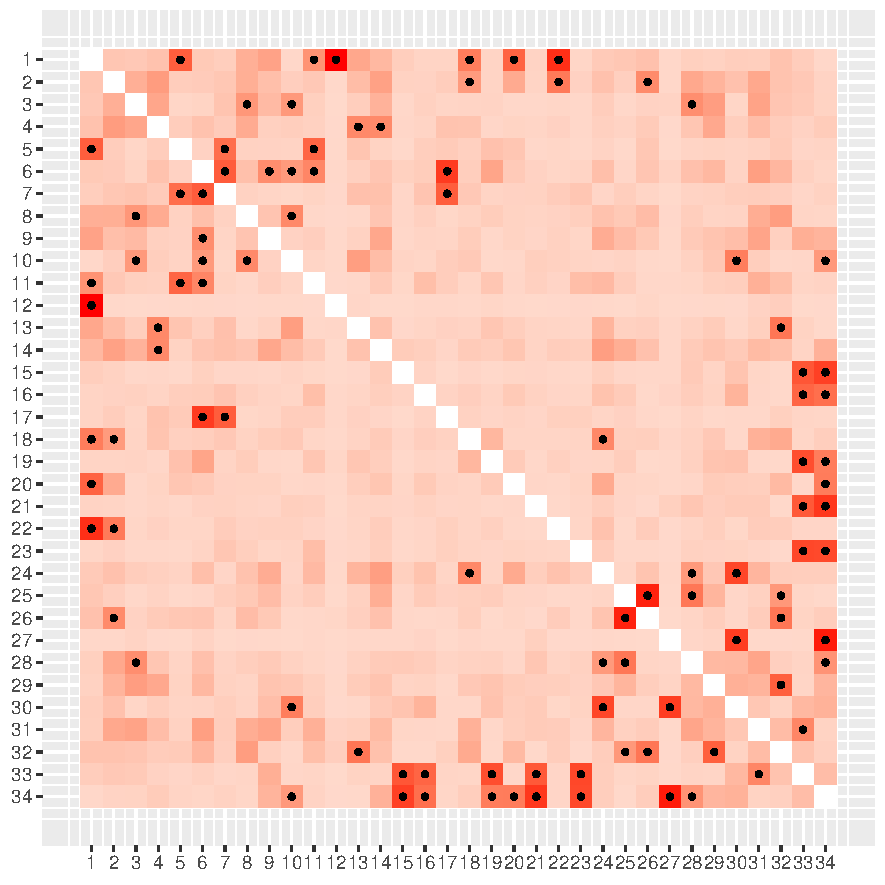
\includegraphics[height=0.8\textheight]{figures/K22-posterior-W.pdf}
		\caption{Posterior Mean $\WW$}
	\end{figure}
\end{frame}

\begin{frame}{Zachary's Karate Club: Results K2} %% TODO
	\begin{center}
		\scriptsize
		\begin{tabular}{cl|rlrrr}
			\toprule
			\multirow{2}{*}{Spec.} &
			\multirow{2}{*}{Param.} &
			\multirow{2}{*}{True}  &
			\multirow{2}{*}{Prior Dist.} &
			\multirow{2}{*}{Post.\ Mean} &
			\multicolumn{2}{c}{$95\%$ Credible Interval} \\
			& & & & & $Q_{2.5\%}$ & $Q_{97.5\%}$ \\
			\midrule
			\multirow{9}{*}{\shortstack[c]{K20\\$T=15$}}
			& $\lambda$                          & $0.1$  & $\Uniform(-1,1)$     & $0.0527$  & $-0.2202$ & $0.3424$   \\
			& $\sigma^2$                         & $5$    & $\InverseGamma(1,1)$ & $45.0312$ & $8.3686$  & $140.6322$ \\
			& $\bbeta_{1,1}$                     & $2$    & $\Normal(0,30)$      & $1.9974$  & $1.5802$  & $2.5150$   \\
			& $\bbeta_{1,2}$                     & $1$    & $\Normal(0,30)$      & $0.8264$  & $-5.0927$ & $8.6789$   \\
			& $\bbeta_{2}$                       & $0.5$  & $\Normal(0,30)$      & $0.6450$  & $0.1342$  & $0.9109$   \\
			& $\ttheta_{\text{\Verb"edges"}}$    & $-3$   & $\Normal(-3,1)$      & $-2.4708$ & $-3.4504$ & $-1.2638$  \\
			& $\ttheta_{\text{\Verb"2-star"}}$   & $0.2$  & $\Normal(0.2,1)$     & $0.7538$  & $0.1035$  & $1.4728$   \\
			& $\ttheta_{\text{\Verb"3-star"}}$   & $-0.1$ & $\Normal(-0.1,1)$    & $-0.3072$ & $-0.9901$ & $-0.0301$  \\
			& $\ttheta_{\text{\Verb"triangle"}}$ & $0.3$  & $\Normal(0.3,1)$     & $0.2463$  & $-0.6884$ & $1.1994$   \\
			\midrule
			\multirow{9}{*}{\shortstack[c]{K21\\$T=12$}}
			& $\lambda$                          & $0.1$  & $\Uniform(-1,1)$     & $0.0216$  & $-0.3382$ & $0.3432$   \\
			& $\sigma^2$                         & $5$    & $\InverseGamma(1,1)$ & $43.4672$ & $7.9732$  & $178.8634$ \\
			& $\bbeta_{1,1}$                     & $2$    & $\Normal(0,30)$      & $2.0573$  & $1.6866$  & $2.4233$   \\
			& $\bbeta_{1,2}$                     & $1$    & $\Normal(0,30)$      & $1.0191$  & $-3.1973$ & $4.3400$   \\
			& $\bbeta_{2}$                       & $0.5$  & $\Normal(0,30)$      & $0.6581$  & $0.0032$  & $1.3475$   \\
			& $\ttheta_{\text{\Verb"edges"}}$    & $-3$   & $\Normal(-3,1)$      & $-2.4819$ & $-3.3739$ & $-1.3568$  \\
			& $\ttheta_{\text{\Verb"2-star"}}$   & $0.2$  & $\Normal(0.2,1)$     & $0.7527$  & $0.1402$  & $1.5161$   \\
			& $\ttheta_{\text{\Verb"3-star"}}$   & $-0.1$ & $\Normal(-0.1,1)$    & $-0.2971$ & $-0.9783$ & $-0.0365$  \\
			& $\ttheta_{\text{\Verb"triangle"}}$ & $0.3$  & $\Normal(0.3,1)$     & $0.2581$  & $-0.7139$ & $1.2428$   \\
			\bottomrule
		\end{tabular}
	\end{center}
\end{frame}

\begin{frame}{Zachary's Karate Club: Results Summary}
	\begin{itemize}
		\item
			A larger $\lambda$ leads to a more volatile estimation of the parameters.
		\item
			A more complex \acrshort{ergm} does not necessarily perform better,
			this is perhaps due to high correlation in some dimensions in the posterior of $\ttheta$.
			In fact, the correlation between posterior $\ttheta_{\text{\Verb"kstar(2)"}}$ and $\ttheta_{\text{\Verb"kstar(3)"}}$ is about $0.8$,
			which is to be expected.
	\end{itemize}
\end{frame}

\section{Conclusion}

\begin{frame}{Conclusion}
	\begin{itemize}
		\item
			In this paper,
			we present a novel method to estimate \acrshort{sar} models
			that introduces a network formation process/probability as a prior distortion on network $\WW$.
		\item
			This approach brings two main benefits:
			\begin{enumerate}
				\item
					It is a natural extension of high-dimensional methods
					to more complex restrictions.
				\item
					It has more economic interpretability compared to common high-dimensional restrictions
					and can be easily extended for different scenarios.
			\end{enumerate}
		\item
			The main difficulty lies in efficient sampling algorithms
			and a data set that is sufficiency informative.
		\item
			The effect of the most interest $\lambda$ cannot be reliably recovered.
	\end{itemize}
\end{frame}

\appendix

\section{\acrshort{ergm} Terms}

\begin{frame}{\acrshort{ergm} Terms}
	\begin{table}[t]
	\centering
	\begin{tabular}{l|l}
		\toprule
		Term & Description \\
		\midrule
		\Verb"edges"    & number of edges \\
		\Verb"kstar(2)" & number of $2$-stars \\
		\Verb"kstar(3)" & number of $3$-stars \\
		\Verb"triangle" & number of triangles \\
		\Verb"ctriad"   & number of cyclic triples \\
		\Verb"ttriad"   & number of transitive triples \\
		\bottomrule
	\end{tabular}
	\caption{Implemented \acrshort{ergm} terms.}
	\label{tab:ergm-terms}
\end{table}

\end{frame}

\section{Decision Theoretic Discussion}

\begin{frame}{Loss Functions}
	\begin{enumerate}
		\item
			A common loss function is the mean-square loss.\\
			This loss corresponds to the posterior mean decision.
		\item
			A more reasonable loss for in our case for $\WW$ is miss-categorization loss:
			\begin{align*}
				L(\hat\WW,\WW_0) = \#\{(i,j):\hat\WW_{i,j}\neq(\WW_{0})_{i,j}\}.
			\end{align*}
			This loss corresponds to the decision:
			\begin{align*}
				\hat\WW_{i,j} = \one
				\left\{
				\pr((\WW_0)_{i,j}=1\given\{\yy_{t}\}) \geq 0.5
				\right\}.
			\end{align*}
	\end{enumerate}
\end{frame}

\end{document}
